\chapter{Podržano učenje}

Strojno učenje \engl{Machine learning} je grana umjetne inteligencije \engl{artificial inteligence} koje se može definirati kao skup metoda koje u podatcima mogu automatski otkrivati obrasce, i potom te otkrivene obrasce iskorištavati pri budućem predviđanju podataka, ili obavljati druge zadatke odlučivanja u prisustvu nesigurnosti \cite{CupicUvod}. Drugim riječima, bez eksplicitnog programiranja moguće je napraviti sustave koji funkcioniraju kao ljudski mozak - imaju pristup podatcima, koriste ih za učenje i samim time bolje razumiju entitete, domene i veze između podataka. 

Strojno učenje dijeli se na 3 podvrste: nadzirano učenje, nenadzirano učenje i podržano (ojačano) učenje. Nadzirano učenje \engl{supervised learning} karakterizira učenje modela nad testnim podatcima koji su označeni. Model točno zna da za određeni ulaz mora vratiti izlaz koji je istovjetan unaprijed pridruženoj oznaci. Algoritam mjeri točnost kroz funkciju gubitka, prilagođavajući se sve dok se izračunata razlika izlaza modela i stvarnog izlaza (pogreška) ne smanji do određene mjere. S druge strane, u nenadziranom učenju \engl{unsupervised learning} posjedujemo podatke bez zadanog izlaza - podatci su dani bez ciljne vrijednosti i u tim situacijama treba pronaći određenu pravilnost. Postupci poput grupiranja, smanjenja dimenzionalnosti, otkrivanja veza između primjeraka... pripadaju nenadziranom učenju.

Posebna i nama najzanimljivija podvrsta strojnog učenja jest podržano učenje \engl{reinforcement learning}. Podržano učenje bavi se optimizacijom ponašanja agenta koji je u interakciji s okolinom (u kojoj se nalazi) i koji izvršava akcije na temelju informacija koje dobiva iz okoline. Agent pri svakom koraku od okoline dobiva povratnu informaciju u obliku nagrade ili kazne. Za razliku od prethodne dvije navedene podvrste koje mapiraju ulazne podatke na određeni format izlaza, u podržanom učenju je najizraženije učenje iz iskustva koje je čovjeku i drugim živim bićima veoma blisko.

\section{Ključni koncepti}
\label{chap:kljucni-koncepti}

Za potpuno razumijevanje podržanog učenja, bitno je u navesti i pojasniti ključne koncepte i terminologiju. Okolina \engl{environment} označava svijet u kojem se agent nalazi i s kojim interaktira. Stanje $s_t$ \engl{state} reprezentira kompletni opis okoline u određenom trenutku $t$. S druge strane, opservacija okoline $o_t$ \engl{observation} predstavlja prilagođeni i ograničeni opis okoline koji agent dobije u nekom trenutku. Kada se agent nađe u nekom stanju $s_t$ i kada od okoline dobije opservaciju $o_t$, tada agent poduzima akciju $a_t$ \engl{action} i samim time u idućem vremenskom koraku inicira promjenu stanja $s_{t+1}$ i opservacije okoline $o_{t+1}$. 

Način na koji agent odabire akciju iz skupa svih dostupnih akcija naziva se politika \engl{policy}. Politika ovisi o parametrima modela $\theta$ i može biti deterministička $\mu_{\theta}$ ili stohastička $\pi_{\theta}$. Veza između akcije, politike i stanja prikazana je izrazima \ref{md:policy}. U našem slučaju koristiti ćemo politike koji su zapravo duboki modeli - aproksimacije funkcije odluke čiji se parametri uče optimizacijskim algoritmima.  

\begin{equation}
    \begin{gathered}
    \label{md:policy}
    a_t = \mu_{\theta}(s_t) \\
    a_t \sim \pi_{\theta}(\cdot \mid s_t)
    \end{gathered}
\end{equation}

\bigskip

Nadalje, putanja $\tau$ \engl{trajectory} je pojam koji označava niz stanja i pripadajućih akcija i predstavljen je izrazom \ref{md:trajectory}. Interakcija s okolinom započinje u trenutku $t = 0$ kada pomoću funkcije za inicijalizaciju okoline $\rho_0$ poštujući pravila okoline, nasumično generiramo stanje $s_0$.

\begin{equation}
    \label{md:trajectory}
    \tau = (s_0, a_0, s_1, a_1, ...)
\end{equation}

\bigskip

Najvažnija i najkorisnija informacija koju agent dobiva od okoline jest nagrada $r_t$ \engl{reward} koju generira funkcija $R$ \engl{reward function} i koja u obzir uzima trenutno i iduće stanje te akciju koja je izazvala promjenu stanja. Povezanost između generiranja iznosa nagrade i same nagrade prikazana je izrazom \ref{md:reward}.

\begin{equation}
    \label{md:reward}
    r_t = R(s_t, a_t, s_{t+1})
\end{equation}

\bigskip

Želimo dobiti što bolji pregled koliko su bile dobre akcije koje je agent poduzeo. Tu informaciju možemo predstaviti na dva različita načina. Sumom nekorigiranih nagrada zbrajamo samo nagrade koje su dobivene u fiksnom vremenskom intervalu $T$ (izraz \ref{md:undiscounted-return}). Na taj način dobivamo informaciju o tome kolika je bila prosječna nagrada u zadnjih $T$ koraka. Ako pak želimo pokazati da su nam nagrade u trenutnom stanju vrjednije nego nagrade koje ćemo dobiti u budućim stanjima, moramo uvesti korekcijski faktor (diskontni faktor) $\gamma \in (0,1)$ \engl{discount factor}. Navedeni pristup sumiranja korigiranih nagrada prikazan je izrazom \ref{md:discounted-return}.

\begin{equation}
    \label{md:undiscounted-return}
    R(\tau) = r_0 + r_1 + ... + r_T = \sum_{t=0}^{T}r_t
\end{equation}

\begin{equation}
    \label{md:discounted-return}
    R(\tau) = r_0 + \gamma \cdot r_1 + \gamma^2 \cdot t_2 + \gamma^3 \cdot t_3 + ... = \sum_{t=0}^{\infty}\gamma^t r_t
\end{equation}

\bigskip

U našem slučaju agent interaktira sa stohastičkom okolinom i stoga funkciju politike \engl{policy function} (izraz \ref{md:policy-function}) predstavljamo kao probabilističku funkciju koja u obzir uzima stanje i akciju, i vraća vjerojatnost poduzimanja dane akcije $a_t$ u stanju $s_t$.

\begin{equation}
    \label{md:policy-function}
    \pi(s, a) = P(a_t = a \mid s_t = s)
\end{equation}

\bigskip

Za slučaj kada agent odabire putanju $\tau$ koja je u skladu sa politikom $\pi$ počevši od stanja $s$, moguće je procijeniti ukupnu očekivanu nagradu. Riječ je o funkciji vrijednosti stanja \engl{value function} (izraz \ref{md:value-function}) koja nam u suštini govori koliko je dobro biti u određenom stanju poštujući politiku.

\begin{equation}
    \label{md:value-function}
    V^{\pi}(s) = \E_{\tau \sim \pi} \left[ {R(\tau) \mid s_0 = s} \right]
\end{equation}

\bigskip

S druge strane, imamo funkciju vrijednosti stanja i akcije \engl{action-value function} (izraz \ref{md:action-value-function}) koja predstavlja ukupnu očekivanu nagradu za slučaj da se agent nalazi u stanju $s$ i poduzme akciju $a$ (koja možda nije dio politike) i zatim uvijek postupa prema politici $\pi$.

\begin{equation}
    \label{md:action-value-function}
    Q^{\pi}(s,a) = \E_{\tau \sim \pi} \left[ {R(\tau) \mid s_0 = s, a_0 = a} \right]
\end{equation}

\bigskip

% TODO na sve ovo dodati literaturu https://spinningup.openai.com/en/latest/spinningup/rl_intro.html i http://java.zemris.fer.hr/nastava/ui/rl/rl-20200401.pdf

Dakle, cilj podržanog učenja jest pronaći optimalnu funkciju vrijednosti stanja ili funkciju vrijednosti stanja i akcije (ovisno o vrsti algoritma) te na taj način dobiti optimalnu politiku koja maksimizira ukupnu (kumulativnu) nagradu. U svakom koraku interakcije agenta s okolinom, agent prima opis stanja okoline u kojoj se nalazi. S obzirom na to stanje, izvršava akciju koja vrši neku promjenu nad okolinom i prebacuje ju u novo stanje. Agent prima povratnu informaciju od okoline koja reprezentira koliko je odabrana akcija dobra. Opisana interakcija agenta i okoline prikazana je na slici \ref{fig:rl}.

\begin{figure}[H]
    \centering
    \frame{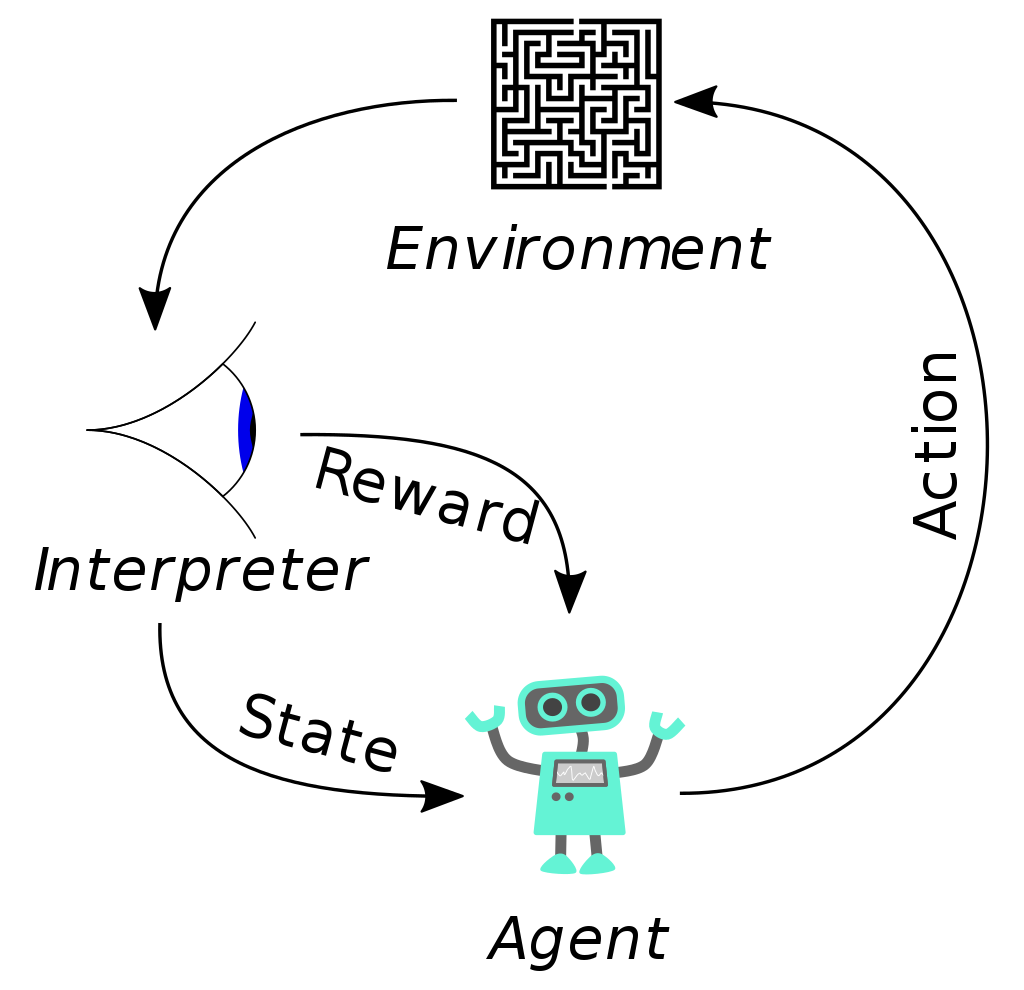
\includegraphics[width=8cm]{assets/rl_diagram.png}}
    \caption{Ciklus interakcije agenta s okolinom \cite{wikiRL}}
    \label{fig:rl}
\end{figure}

\section{Duboki modeli}
\label{chap:duboki-modeli}

Duboko učenje \engl{Deep learning} jest tip strojnog učenja (točnije, podskup strojnog učenja) koje nastoji oponašati način zaključivanja i obrasce koje ljudski mozak koristi za učenje i donošenje odluka. Veliku ulogu u cijeloj ideji dubokog učenja imaju duboke neuronske mreže \engl{deep neural networks, DNN} pomoću kojih se povezivanjem više slojeva procesnih elemenata (čvorova, neurona), dobivaju duboki modeli koji su sposobni učiti i baratati s podatcima kompozitne strukture. Primjenom dubokih modela dolazimo do slijeda naučenih nelinearnih transformacija kojima aproksimiramo funkciju odluke, učimo mapiranje između ulaznih podataka i izlazih podataka, te nastojimo postići dobru generalizaciju nad stvarnim podatcima \cite{DLBook}. 

\subsection{Unaprijedni potpuno povezani modeli}

Unaprijedni potpuno povezani modeli \engl{Fully connected neural network} (poznatiji i pod nazivom višeslojni perceptron \engl{Multi-layer perceptron}) sastoje se od lanaca potpuno povezanih slojeva. Svaki neuron iz prethodnog sloja povezan je s neuronom idućeg sloja. 

Sastoje se od tri vrste slojeva - ulaznog sloja, izlaznog sloja i skrivenih slojeva. Ulaznom sloju dovode se podatci koje je potrebno obraditi. Izlaz neuronske mreže (u najosnovnijem obliku) predstavljen je logitima \engl{logits} - vektorima logaritama nenormaliziranih vrijednosti. Specifičnije, za slučaj da želimo provesti klasifikaciju podataka ili drugačije organizirati izlazne vrijednosti na izlaz dodajemo posebni sloj (npr. \textit{Softmax} funkcija za klasifikaciju). Samo su ulaz i izlaz specificirani dimenzijama. Model ima slobodu da iskoristi skrivene slojeve na način koji osigurava najbolju aproksimaciju funkcije. Neuronskim mrežama želimo izgraditi modele koji nisu linearno odvojivi i zato koristimo nelinearnu aktivacijsku funkciju - najčešće ReLU (Rectified Linear Unit). Svaki od slojeva modelira jednu nelinearnu transformaciju.

Slika \ref{fig:nn} \cite{NNsvg} prikazuje arhitekturu potpuno povezanog modela koji je sastavljen od sveukupno 4 potpuno povezana sloja - ulaznog (dimenzije 4), izlaznog (dimenzije 2) i dva skrivena sloja (svaki dimenzije 8). Kodom \ref{lst:fcn} prikazana je implementacija navedenog modela u biblioteci \textit{PyTorch}.

\begin{figure}[H]
    \centering
    \frame{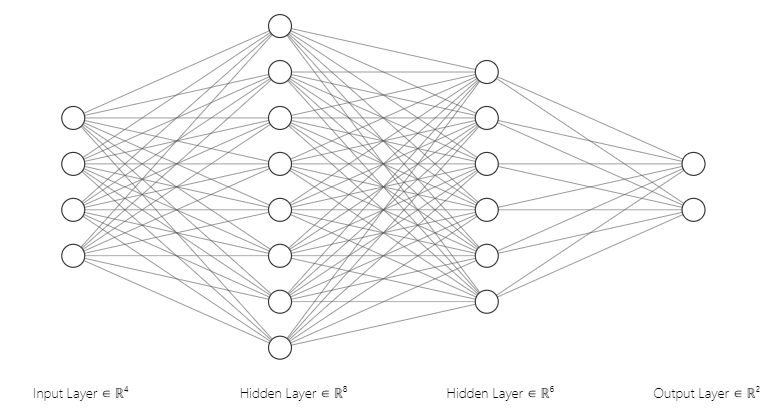
\includegraphics[width=11cm]{assets/nn.png}}
    \caption{Arhitektura potpuno povezanog modela}
    \label{fig:nn}
\end{figure}

\begin{listing}[H]
    \caption{Implementacija potpuno povezanog modela na slici \ref{fig:nn} koristeći biblioteku \textit{PyTorch}}
    \inputminted{python}{snippets/fcn.py}
    \label{lst:fcn}
\end{listing}

\subsection{Konvolucijski modeli}

Konvolucijski modeli \engl{Convolutional neural networks} su modeli koji uz potpuno povezane slojeve imaju najmanje jedan konvolucijski sloj \engl{convolution layer}. Osim spomenutih slojeva, konvolucijski modeli sadrže i slojeve sažimanja \engl{pooling layers}, slojeve u kojima provodimo nelinearnost podataka te sloj koji višedimenzionalni ulaz pretvara u jednodimenzionalni i pritom priprema podatke za obradu u potpuno povezanim slojevima \engl{flatten layer}.

Operacija konvolucije provodi se nad ulazom i jezgrom \engl{kernel} (slobodnim parametrima koje učimo) gdje kao rezultat dobivamo mapu značajki koja pokazuje gdje se koja značajka nalazi u ulaznim podatcima (npr. slici). Dimenzije mapa značajki i njihovu robusnost korigiramo korištenjem atributa koraka konvolucije \engl{stride} i nadopunjavanja ulaznih podataka \engl{padding}. Slično konvolucijskom sloju, sloj sažimanja odgovoran je za smanjenje prostora značajki (smanjenje dimenzionalnosti podataka) i dodatno za izdvajanje dominantnih značajki. Razlikujemo dvije vrste sažimanja: sažimanje maksimalnom vrijednosti \engl{max pooling} i sažimanje srednjom vrijednosti \engl{average pooling}. Prilikom sažimanja značajki maksimalnom vrijednošću u obzir uzimamo samo značajku najveće vrijednosti te na taj način uklanjamo šum ulaza i potencijalno biramo značajku najveće važnosti.

Korištenje konvolucijskih modela biti će nam iznimno potrebno u situacijama kada su ulazni podatci u formi slike, odnosno kada su nam važne lokalne interakcije između ulaznih podataka (piksela) te njihova vremenska i prostorna ovisnost.

Slika \ref{fig:cnn} \cite{NNsvg} prikazuje jednostavni konvolucijski model koji se sastoji od konvolucijskog sloja, sloja sažimanja maksimalnom vrijednosti, sloja koji $3$-dimenzionalne podatke pretvara u $1$-dimenzionalne, te dva potpuno povezana sloja. Ulaz u konvolucijski sloj predstavlja RGB slika (3 kanala) dimenzije $32 \times 32$. Primjenom konvolucije (veličina jezgre 3, korak 3, nadopuna 1) izvlačimo 18 kanala značajki dimenzije $32 \times 32$ (dimenzija se nije promijenila iz razloga što nadopunjavamo ulaz). Primjenom sažimanja maksimumom (veličina jezgre 2, korak 2) smanjujemo broj značajki na dimenziju $16 \times 16$. Prvi potpuno povezani sloj na svoj ulaz dobije vektor dimenzije $4608$ kojeg pretvara u vektor izlaza dimenzije $64$. Posljednji potpuno povezani sloj koji je ujedno i posljednji sloj u ovom konvolucijskom modelu za izlaz predaje vektor dimenzije $10$. Isječak koda koji prikazuje implementaciju jednostavnog konvolucijskog modela koristeći bibilioteku \textit{PyTorch} prikazan je kodom \ref{lst:cnn}.

\begin{figure}[H]
    \centering
    \frame{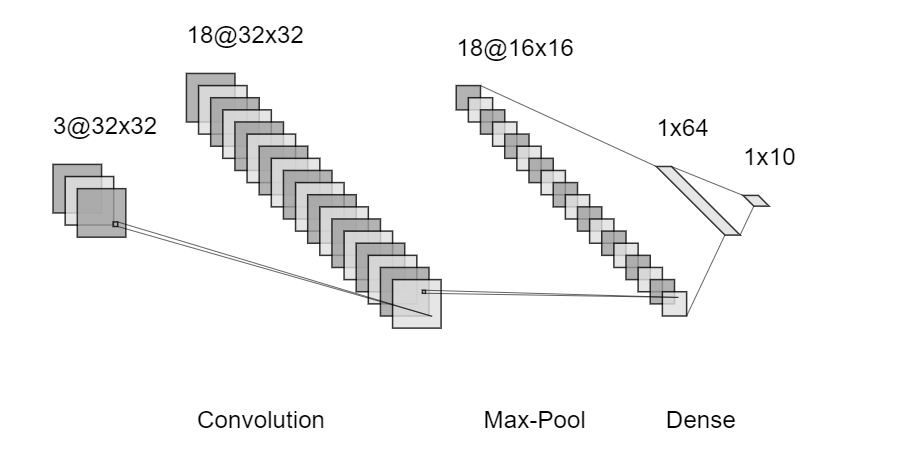
\includegraphics[width=11cm]{assets/cnn.png}}
    \caption{Arhitektura konvolucijskog modela}
    \label{fig:cnn}
\end{figure}

\begin{listing}[H]
    \caption{Implementacija konvolucijskog modela na slici \ref{fig:cnn} koristeći biblioteku \textit{PyTorch}}
    \inputminted{python}{snippets/cnn.py}
    \label{lst:cnn}
\end{listing}

\section{Algoritmi podržanog učenja}

Način na koji pristupamo problemu pronalaženja optimalne politike prvenstveno ovisi o informacijama koje okolina pruža agentu i o tome je li poznato unutarnje djelovanje okoline - ima li agent pristup modelu okoline (pristup internoj funkciji okoline koja predviđa prijelaze stanja i nagrade). Pritom razlikujemo pristupe koji su temeljeni na modelu - poznaju funkciju predviđanja \engl{model-based methods} i pristupe koji okolinu promatraju kao crnu kutiju i pritom nisu upoznati s njenim pravilima niti principima funkcioniranja \engl{model-free methods}.

Podržano učenje često pokušava riješiti probleme iz svakodnevnog života čiji temeljni model okruženja nije dostupan ili ga je pak teško implementirati. Samim time, nije u potpunosti praktično razmatrati postupke koji se temelje na modelu, koji svoje korake mogu unaprijed planirati i pritom ne zahtijevaju interakciju s okolinom. S druge strane, metode koje u obzir ne uzimaju model moraju jedino znati točnu reprezentaciju stanja okoline i skup akcija koje agent može poduzimati. Gruba podjela algoritama podržanog učenja prikazana je na slici \ref{fig:rl-algorithms}

%% TODO dodati dio oko on policy i off policy algoritama (učenje s isključenom politikom)

\begin{figure}[H]
    \centering
    \frame{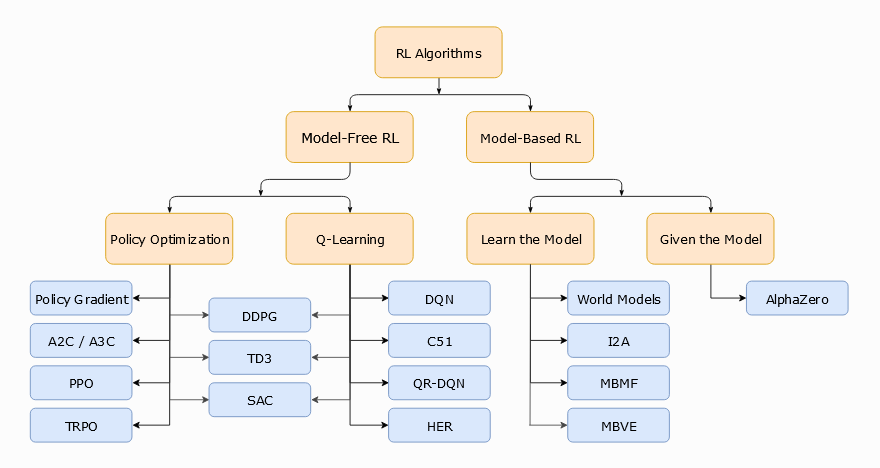
\includegraphics[width=14cm]{assets/rl-algorithms.png}}
    \caption{Gruba podjela algoritama podržanog učenja \cite{RLAlgos}}
    \label{fig:rl-algorithms}
\end{figure}

% https://spinningup.openai.com/en/latest/spinningup/rl_intro2.html

% dodati literaturu https://www.fer.unizg.hr/_download/repository/SU-2020-02-OsnovniKoncepti.pdf

Svaki algoritam strojnog učenja definiran modelom, gubitkom i metodom optimizacije. Model je postupak obrade (odnosno skup funkcija) sa slobodnim parametrima koji za određen ulaz daje pripadajući izlaz. Gubitak je mjera koja na formaliziran način vrednuje slobodne parametre modela, odnosno pokazuje u kojoj mjeri se mi ne slažemo s onim što je model predstavio kao izlaz. Metoda optimizacije (optimizacijski postupak) jest način na koji pronalazimo optimalne parametre koji su važni kako bi minimizirali prethodno navedenu komponentu - gubitak. Navedene tri glavne komponente biti će važno napomenuti pri svakom predstavljaju algoritma jer su to glavne odrednice pri analizi algoritama strojnog učenja.

\subsection{Q učenje}

Osnovna inačica algoritma naziva se Q učenje \engl{Q Leaning}. Pripada skupini algoritama s isključenom politikom, jer uči iz akcija koje nisu dio trenutne politike. Algoritam procjenjuje kvalitetu \engl{quality} poduzimanja određene akcije i govori koliko je ona korisna pri dobivanju buduće nagrade. Osnovna inačica algoritma koristi jednostavnu strukturu podataka zvanu Q tablica \engl{Q Table} i pogodna je za korištenje u okolinama s ograničenim i relativno malim brojem stanja i akcija. 

Q tablica sastoji se od svih mogućih uređenih dvojki $[stanje, akcija]$ i pridruženih vrijednosti (q vrijednosti) koje su prvotno inicijalizirane na $0$. Izgled ove strukture prikazan je na slici \ref{fig:q-learning} (gornja struktura, pridružena algoritmu Q učenja). Učenje se provodi iterativno: odabire se i izvršava akcija koja u trenutnom stanju ima najveću q vrijednost, izračunava se nagrada, i na posljetku, izračunava se nova q vrijednost koristeći Bellmanovu jednadžbu \ref{md:bellman}. Na kraju učenja, q tablica nam zapravo pokazuje koja je najbolja akcija koju možemo poduzeti u određenom stanju.

Kako bi optimizirao politiku, agent ima opciju istraživanja novih stanja i maksimiziranja svoje ukupne nagrade. Mora pronaći kompromis između istraživanja (odabira nasumične akcije) \engl{exploration} i odabira akcije s najvećom q vrijednošću \engl{exploitation}. Najbolja strategija bila bi uvesti hiperparametar $\epsilon$ koji označava vjerojatnost nasumičnog odabira akcije (umjesto odabira najbolje akcije) kojim bi se model kratkoročno žrtvovao ali sve u svrhu donošenja najbolje cjelokupne odluke u budućnosti. Navedena tehnika naziva se \textit{epsilon-greedy exploration strategy}.

Uzevši u obzir prethodno navedene činjenice, pri početku treniranja akcije biramo nasumično kako bi agent mogao istražiti okolinu. Daljnjim treniranjem, smanjujemo vrijednost hiperparametra $\epsilon$ i samim time smanjujemo utjecaj strategije nasumičnog istraživanja i povećavamo utjecaj odabira akcije s najvećom Q vrijednošću. Na taj način, agent sve više koristi informacije koje je skupio prethodnim istraživanjem. 

%% https://www.assemblyai.com/blog/reinforcement-learning-with-deep-q-learning-explained/

%% TODO literatura za sliku 

\begin{equation}
    \label{md:bellman}
    Q(s_t, a_t) = Q(s_t, a_t) + \alpha \left[ r_t + \gamma \max_a Q(s_{t+1}, a) - Q(s_t, a_t) \right]
\end{equation}

\bigskip

Prikazana Bellmanova jednadžba \ref{md:bellman} iskazuje ukupnu korisnost poduzimanja akcije $a_t$ kada se nalazimo u stanju $s_t$. Sastoji se od nekoliko hiperparametara. Koeficijent $\alpha$ označava stopu učenja \engl{learning rate}, parametar s kojim iskazujemo u kojoj mjeri želimo da nova vrijednost pridonese ukupnom zbroju vrijednosti. Koeficijent $\gamma$ predstavlja korekcijski faktor \engl{discount factor} koji je već predstavljen u poglavlju \nameref{chap:kljucni-koncepti}. Dakle, ažurirana procjena vrijednosti akcije sastoji se od zbroja trenutne procjene i skalirane korekcijske vrijednosti \engl{temporal difference error}. Korekcijska vrijednost je razlika između ciljane vrijednosti q učenja \engl{temporal difference target} te procjene trenutne vrijednosti akcije i u suštini govori u kojoj mjeri se trenutna vrijednost treba ažurirati kako bi smanjili odstupanje između procjene q vrijednosti susjednih stanja. Ukupnu nagradu nastojimo procijeniti zbrojem trenutne nagrade (dobivene izvođenjem akcije $a_t$) i skalirane optimalne vrijednosti buduće akcije (ciljane politike). 

Kao što je već rečeno, algoritam Q učenja pripada skupini algoritama s isključenom politikom i to je upravo vidljivo iz dijela Bellmanove jednadžbe. Pri postupku učenja, neovisno o tome koja se trenutno politika slijedi, pri računanju uzimamo u obzir buduću akciju čija je Q vrijednost optimalna. Ta akcija može, ali i ne mora biti dio politike koja se trenutno slijedi. 

%% https://www.youtube.com/watch?v=0iqz4tcKN58

%% http://databookuw.com/databook.pdf

\begin{figure}[H]
    \centering
    \frame{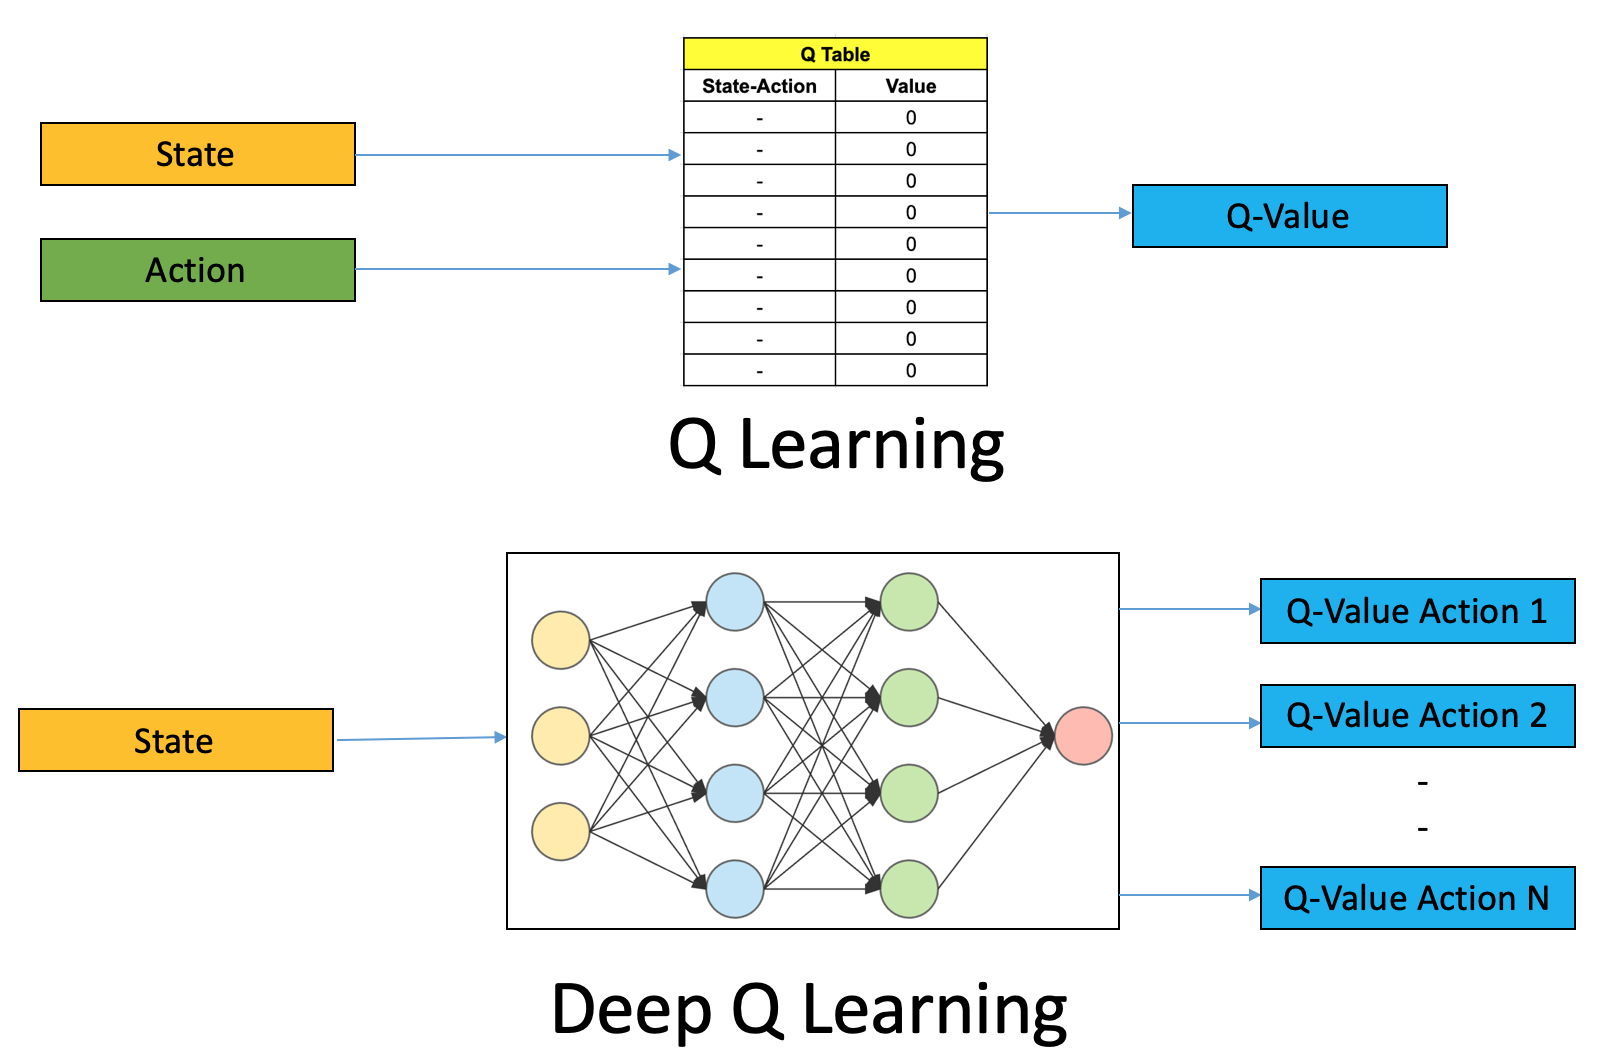
\includegraphics[width=12cm]{assets/q-learning.png}}
    \caption{Razlika u strukturama koje koriste Q učenje i Duboko Q učenje}
    \label{fig:q-learning}
\end{figure}

\subsection{Duboko Q učenje}

Korištenje q tablica nije pogodno za kompleksne okoline, okoline s velikim brojem stanja i akcija. U takvim okolinama koristi se inačica Q učenja, duboko Q učenje, čija je ideja, opis, niz objašnjenih formula i algoritam predstavljen u članku \cite{DQL}. Osnovna ideja ovog algoritma jest naučiti duboki model da za određeno stanje okoline na ulazu, generira skup svih akcija i pripadajućih vrijednosti funkcije stanja i akcije, i pritom izabere akciju s pripadajućom najvećom vrijednošću $Q(s, a)$ funkcije \ref{md:action-value-function}. Slika \ref{fig:q-learning} upravo pokazuje tu razliku u korištenim strukturama za generiranje i procjenu vrijednosti funkcije kvalitete.

U procesu učenja koriste se 2 neuronske mreže jednake arhitekture i različitih vrijednosti težina parametara. Razlikujemo neuronsku mrežu koja prati trenutnu politiku (i pritom provodi stalno ažuriranje parametara) \engl{policy neural network, online neural network} i neuronsku mrežu koja prati ciljanu politiku \engl{target neural network}. Svakih $N$ koraka vrijednosti težina parametara ciljne neuronske mreže zamjenjuju se vrijednostima parametara mreže koja prati trenutnu politiku. Samo treniranje (optimizacija parametara) provodi se nad mrežom koja prati trenutnu politiku. Korištenje dviju neuronski mreža pospješuje stabilnost i učinkovitost procesa učenja. Druga neuronska mreža služi nam pri izračunu ciljane vrijednosti q učenja. Njene parametre ne optimiziramo. Samim time osigurava se da izračun ciljane vrijednosti q učenja bude stabilan, sve dok se njeni parametri zamijene parametrima učene mreže.

Funkciju kvalitete $Q(s, a)$ aproksimirat ćemo neuronskom mrežom. Stoga, prikladno ju je zapisati kao funkciju parametriziranu težinama neuronske mreže, $\theta$ \ref{md:dqn-theta}. Nadalje, operacija ažuriranja vrijednosti funkcije akcije pomoću neuronskih mreža može se izraziti jednadžbom \ref{md:dqn-bellman}. Funkcija gubitka \ref{md:dqn-loss} predstavljena je kao razlika između ciljane vrijednosti q učenja (koju aproksimira ciljna neuronska mreža u ovisnosti o njenim težinama $\theta^-$) te procjene trenutne vrijednosti akcije (koju aproksimira trenutna neuronska mreža u ovisnosti o njenim težinama $\theta$).

\begin{equation}
    \label{md:dqn-theta}
    Q(s, a) \approx Q(s, a; \theta)
\end{equation}

\begin{equation}
    \label{md:dqn-bellman}
    Q(s_t, a_t; \theta) = Q(s_t, a_t; \theta) + \alpha \left[ r_t + \gamma \max_a Q(s_{t+1}, a; \theta^-) - Q(s_t, a_t; \theta) \right]
\end{equation}

\begin{equation}
    \label{md:dqn-loss}
    \mathcal{L}(\theta) = \left[ r_t + \gamma \max_a Q(s_{t+1}, a; \theta^-) - Q(s_t, a_t; \theta) \right]
\end{equation}

\bigskip

%% TODO spomenuti hubert loss a ne MSE

Grupno \engl{batch} učenje pozitivnije utječe na optimizacijski postupak od pojedinačnog učenja, zbog preciznijeg gradijenta. Uzorci za grupu trebali bi biti odabrani slučajnim uzorkovanjem kako bi bili nezavisni (želimo odrediti nepristranu procjenu gradijenta). To nam je motivacija za uvođenje metode ponavljanja iskustva \engl{experience replay}. U spremnik za ponavljanje \engl{replay buffer} pohranjuju se sve akcije, stanja i nagrade koje je agent poduzeo od početka. Konačno, pri svakoj iteraciji postupka učenja, iz liste se izvlači određeni broj uzoraka (grupa).

%% http://www.zemris.fer.hr/~ssegvic/du/du3optimization.pdf

Algoritam \ref{fig:dql-algorithm} prikazuje pseudokod dubokog Q učenja s metodom ponavljanja iskustva, dvije neuronske mreže za aproksimaciju Q funkcija, zamjenu vrijednosti težina parametara, metodu ponavljanja iskustva, izračun funkcije gubitka. 

\begin{figure}[H]
    \centering
    \frame{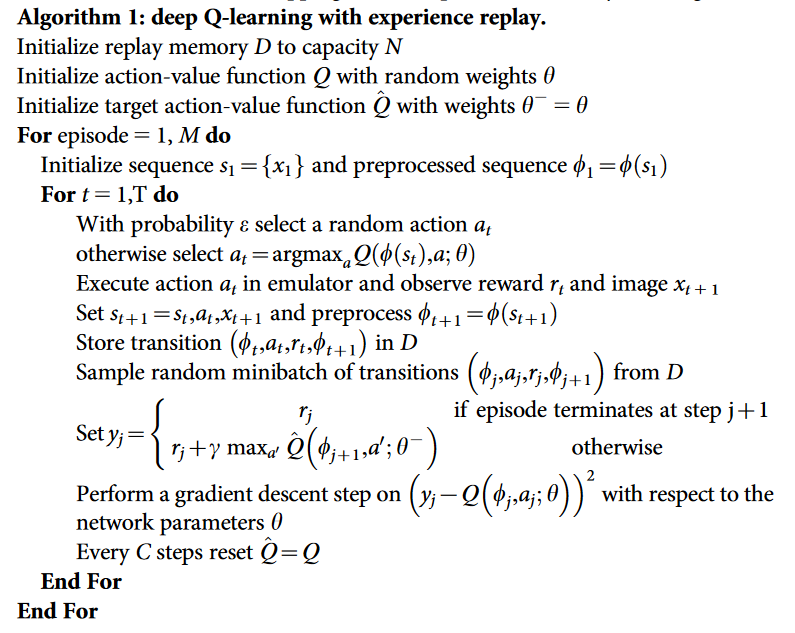
\includegraphics[height=9.5cm]{assets/dql-algorithm.png}}
    \caption{Algoritam dubokog Q učenja s ponavljanjem iskustva}
    \label{fig:dql-algorithm}
\end{figure}

%% TODO lista hiperparametra?!?

\subsection{Dvostruko duboko Q učenje}

Algoritam dubokog Q učenja ima tendenciju precjenjivanja vrijednosti funkcije akcije. Odabir akcije koja ju maksimizira i procjenu njene vrijednosti (u ovisnosti o akciji odabranoj u prethodnom koraku), provodi se samo nad vrijednostima težinskih parametara $\theta^-$ ciljne neuronske mreže, kao što je i prikazano jednadžbom \ref{md:dqn-overest} \cite{DQN-impl}. Precijenjene vrijednosti ne predstavljaju problem u slučajevima kada su sve vrijednosti ravnomjerno uvećane. Međutim, ako precjenjivanje nije ujednačeno, tada bi ono moglo negativno utjecati na kvalitetu rezultirajuće politike, pogotovo u okolinama s većim brojem akcija. Navedeni problem predstavljen je u članku \cite{DDQL} uz potencijalno rješenje u vidu algoritma dvostrukog dubokog Q učenja.

\begin{equation}
    \label{md:dqn-overest}
    \max_a Q(s_{t+1}, a; \theta^-) =  Q(s_{t+1}, \argmax_a Q(s_{t+1}, a, \theta^-); \theta^-)
\end{equation}

\bigskip

Ideja dvostrukog dubokog Q učenja jest smanjiti precjenjivanje vrijednosti funkcije akcije na način da postupke odabira akcije provodi neuronska mreža koja slijedi politiku (s parametrima $\theta$), a izračun funkcije akcije provodi ciljana neuronska mreža (s parametrima $\theta^-$). Modificirana Bellmanova jednadžba prilagođena za provođenje algoritma dvostrukog dubokog Q učenja i gubitak prikazani su jednadžbama \ref{md:ddqn-bellman} i \ref{md:ddqn-loss}.  

\begin{equation}
    \label{md:ddqn-bellman}
    Q(s_t, a_t; \theta) = Q(s_t, a_t; \theta) + \alpha \left[ r_t + \gamma Q(s_{t+1}, \argmax_a Q(s_{t+1}, a, \theta); \theta^-) - Q(s_t, a_t; \theta) \right]
\end{equation}

\begin{equation}
    \label{md:ddqn-loss}
    \mathcal{L}(\theta) = \left[  r_t + \gamma Q(s_{t+1}, \argmax_a Q(s_{t+1}, a, \theta); \theta^-) - Q(s_t, a_t; \theta) \right]
\end{equation}

\bigskip

Cilj opisanog algoritma dvostrukog dubokog Q učenja bio je smanjiti efekt precjenjivanja vrijednosti funkcije akcije pritom ne mijenjajući osnovni kostur algoritma dubokog Q učenja kako bi mogli na jednostavan način usporediti algoritma bez pretjeranog utroška resursa u računanju. Usporedba je pokazala da u okolinama s većim brojem akcija, algoritam dvostrukog dubokog Q učenja postiže bolje rezultate \cite{DDQL}. Algoritam \ref{fig:ddql-algorithm} prikazuje pseudokod dvostrukog dubokog Q učenja s metodom ponavljanja iskustva, dvije neuronske mreže za aproksimaciju q funkcija, zamjenu vrijednosti težina parametara, metodu ponavljanja iskustva, izračun funkcije gubitka. 

\begin{figure}[H]
    \centering
    \frame{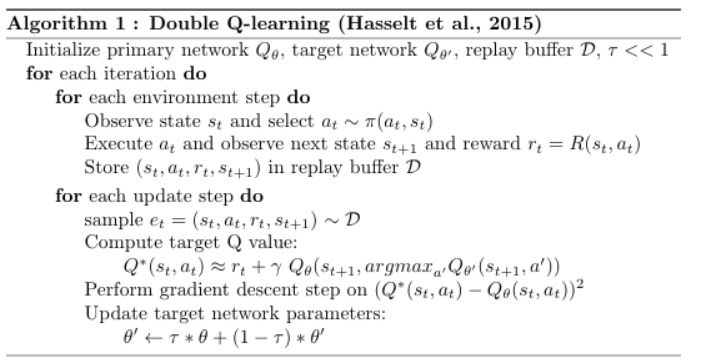
\includegraphics[width=14cm]{assets/ddql-algorithm.png}}
    \caption{Algoritam dvostrukog dubokog Q učenja s ponavljanjem iskustva}
    \label{fig:ddql-algorithm}
\end{figure}

\subsection{Gradijent politike}

%% TODO negdje spomenuti policy gradient na engleski...

Prethodno opisani algoritmi podržanog učenja temeljili su se na aproksimaciji funkcije vrijednosti (kvalitete \engl{quality} pojedine akcije i/ili stanja). Veća vrijednost funkcije vrijednosti označavala je bolju kvalitetu promatrane akcije u određenom stanju. Optimalnu politika pritom implicitno dobijemo izvođenjem niza akcija za koje je model procijenio da su najkvalitetnije. S druge strane, postoje i algoritmi koji se oslanjaju na direktnu aproksimaciju funkcije politike (izraz \ref{md:policy-function}). Funkcija politike vraća vjerojatnosnu distribuciju akcija koje agent može poduzeti ovisno o stanju u kojem se nalazi \cite{tensorflow}. Označena je parametrima $\theta$ i predstavljamo ju izrazom \ref{md:policy-param}.

\begin{equation}
    \label{md:policy-param}
    \pi(s, a) \approx \pi_\theta(s,a) = P(s, a; \theta) 
\end{equation}

\bigskip

Metode zasnovane na politici \engl{policy-based} imaju brojne prednosti: podržavaju stohastičke i determinističke politike, vrlo su učinkoviti u visokodimenzionalnim i kontinuiranim prostorima akcija, te ih karakteriziraju dobra svojstva i izrazito brza konvergencija pod uvjetom korištenja stohastičkog gradijentnog uspona \engl{Stochastic Gradient Ascent} \cite{5.prezza}. U suštini, metode podržanog učenja zasnovane na politici predstavljaju optimizacijski problem. Stohastički gradijentni uspon koristi se zbog ideje maksimiziranja ciljne funkcije politike \engl{policy objective function} $J(\theta)$ definirane izrazom \ref{md:policy-objective-function} koja predstavlja vrijednost očekivanog povrata (kojeg smo izrazom \ref{md:discounted-return} definirali kao sumu diskontiranih nagrada) \cite{https://medium.com/@thechrisyoon/deriving-policy-gradients-and-implementing-reinforce-f887949bd63}. Vrijednost parametara $\theta$ ažurira se u smjeru pozitivnog gradijenta ciljne funkcije politike $J(\theta)$ s korakom učenja $\alpha$ \ref{md:gradient-ascend}. Ažuriranje parametara vrši se na kraju epizode, za razliku od Q učenja gdje su se težine ažurirale na svakom koraku.

\begin{equation}
    \label{md:policy-objective-function}
    J(\theta) = \E_{\tau \sim \pi_\theta} \left[ R(\tau) \right]
\end{equation}

\begin{equation}
    \label{md:gradient-ascend}
    \theta \leftarrow \theta + \alpha \nabla_\theta J(\theta)
\end{equation}

\bigskip

Korištenje neuronskih mreža i derivabilnih aktivacijskih funkcija omogućava pretpostavku da je i politika $\pi_\theta$ koju nastojimo aproksimirati, derivabilna. Na slici \ref{fig:policy-gradient-algos} nalazi se sažeti prikaz algoritama koji se baziraju na gradijentu politike \engl{Policy Gradient} i njihovih izraza za gradijent ciljne funkcije politike.

\begin{figure}[H]
    \centering
    \frame{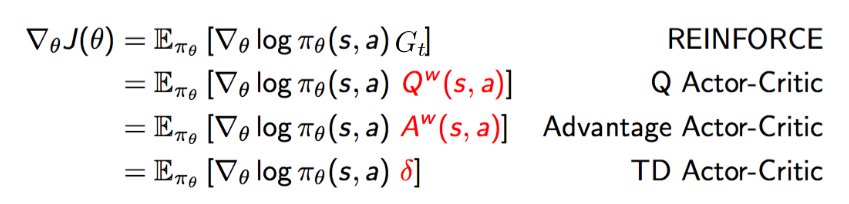
\includegraphics[width=12cm]{assets/policy-gradient-algos.png}}
    \caption{Algoritmi gradijenta politike \cite{https://www.andrew.cmu.edu/course/10-703/slides/Lecture_PG-NatGrad-10-8-2018.pdf}}
    \label{fig:policy-gradient-algos}
\end{figure}

\subsection{Akter-kritičar}

Algoritmi akter-kritičar \engl{Actor-Critic} kombiniraju oba pristupa - aproksimiraju funkciju vrijednosti i funkciju politike. Osnovna ideja jest podijeliti model na dva dijela – akter \engl{Actor}, koji uči parametriziranu politiku i kritičar \engl{Critic}, koji procjenjuje funkciju vrijednosti. Modeli s vremenom (učenjem) u svojoj ulozi postaju sve bolji - akter uči odabirati bolje akcije (počinje učiti politiku), a kritičar postaje bolji u procjeni tih akcija i evaluaciji aktera.

Akter-kritičar algoritmi pripadaju skupini algoritama koji uče s uključenom politikom i nužno je da se do kraja epizode cijelim putem prati odabrana politika. Slika \ref{fig:actor-critic} prikazuje strukturu akter-kritičar algoritama sa specificiranom kritikom u obliku signala greške vremenske razlike (\textit{TD error}) koji je specifičan za svaki pojedini akter-kritičar algoritam. Uzevši u obzir navedeni signal, riječ je o \textit{TD Actor-Critic} algoritmu čija je formula prikazana na slici \ref{fig:policy-gradient-algos}.

\begin{figure}[H]
    \centering
    \frame{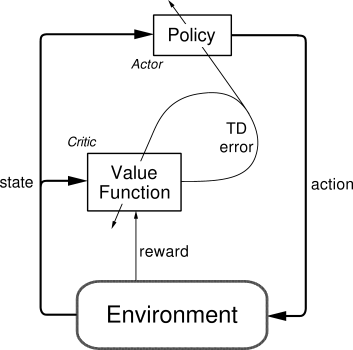
\includegraphics[width=8cm]{assets/actor-critic.png}}
    \caption{Struktura akter-kritičar algoritma \cite{http://www.incompleteideas.net/book/ebook/node66.html}}
    \label{fig:actor-critic}
\end{figure}

Metoda aktor-kritičar ima dobru i intuitivnu analogiju sa svakodnevnim životom i primjerom odrastanja u kojem dijete (koje ima ulogu aktera) istražuje okolinu oko sebe i stalno isprobava nove stvari, dok ga istovremeno njegovi roditelji (koji imaju ulogu kritičara) promatraju, čuvaju i pokušavaju mu dati na znanje koji su njegovi postupci opravdani i dobri, a koji nisu. Dijete zaključuje na temelju povratnih informacija svojih roditelja i prilagođava svoje ponašanje. Kako dijete raste, ono uči koji su postupci dobri i loši, te u suštini uči igrati igru zvanu život.

%% TODO https://theaisummer.com/Actor_critics/

%% TODO https://www.tensorflow.org/tutorials/reinforcement_learning/actor_critic

\subsection{Prednosni akter-kritičar}

Algoritam prednosni akter-kritičar \engl{Advantage Actor Critic} (kraće \textit{A2C}) nasljeđuje sve prednosti osnovnih implementacija akter-kritičar metode. Svrha kritičara je redukcija visoke varijance gradijenta koja je prisutna u običnim metodama zasnovanim na gradijentu politike (npr. u algoritmu gradijenta politike \textit{REINFORCE} prikazanom na slici \ref{fig:policy-gradient-algos} koji koristi kumulativni povrat \ref{md:discounted-return}). 

U algoritmu \textit{A2C} kritičar ocjenjuje trenutnu akciju korištenjem funkcije prednosti \engl{Advantage function}. Ona ukazuje na prednost poduzimanja određene akcije u odnosu na onu koja prati politiku. Izražavamo ju kao razliku vrijednosti akcije (Q vrijednosti) i vrijednosti stanja \ref{md:advantage-function}. Dakle, zadatak kritičara je procijeniti funkciju prednosti i pritom agentu pružiti informaciju o benefitu poduzimanja te akcije u odnosu na akciju koja prati politiku.

\begin{equation}
    \label{md:advantage-function}
    A (s_t, a_t) = Q (s_t, a_t) - V (s_t) 
\end{equation}

\bigskip

Vrijednost akcije aproksimiramo greškom vremenske razlike \ref{md:advantage-function-with-td}. Ako poopćimo trenutnu situaciju da za svaku poduzetu akciju trebamo izračunati vrijednost funkcije prednosti, i uzmemo u obzir da se evaluacija i ažuriranje parametara radi tek na kraju epizode, shvatimo da funkcija $Q (s_t, a_t)$ predstavlja diskontni kumulativni povrat od stanja $t$ pa sve do kraja epizode. Navedena tvrdnja prikazana je izrazom \ref{md:advantage-function-with-return}.

\begin{equation}
    \label{md:advantage-function-with-td}
    A (s_t, a_t) = r_t + \gamma V(s_{t+1}) - V (s_t) 
\end{equation}

\begin{equation}
    \label{md:advantage-function-with-return}
    A (s_t, a_t) = R_t - V (s_t) 
\end{equation}

\bigskip

Akter i kritičar su predstavljeni dubokim modelima. Kritičar ažurira parametre $w$ korištenjem funkcije greške vremenske razlike, dok akter ažurira parametre $\theta$ korištenjem gradijenta politike. Budući da koristimo i aktera i kritičara, ukupna funkcija gubitka izražava se kao zbroj pojedinačnih gubitaka svakog sudionika \ref{md:a2c-loss}. Definirana i opisana funkcija prednosti zajedno s akterovim aproksimacijama vjerojatnosti akcija sudjeluje u maksimiziranju ciljne funkcije politike (odnosno minimiziranju gubitka) i ažuriranju parametara dubokog modela kojim je akter predstavljen \ref{md:a2c-actor-loss} \cite{tensorflow}. Kritičaru želimo da mu je aproksimacija funkcije stanja što bliža stvarnom povratu i zato njegov gubitak predstavljamo izrazom \ref{md:a2c-critic-loss} gdje $L_\delta$ predstavlja huberov gubitak \engl{Hubert loss} \cite{tensorflow}.

\begin{equation}
    \label{md:a2c-loss}
    L = L_{actor} + L_{critic}
\end{equation}

\begin{equation}
    \label{md:a2c-actor-loss}
    L_{actor} = - \sum_{t=1}^{T}\log \pi_\theta (a_t \mid \ s_t) \left[ R_t - V_{w}^{\pi} (s_t) \right]
\end{equation}

\begin{equation}
    \label{md:a2c-critic-loss}
    L_{critic} = L_\delta(R_t, V_{w}^{\pi})
\end{equation}

\bigskip

Pseudokod \textit{A2C} algoritma prikazan je slici \ref{fig:a2c-algorithm}. Dobivena nagrada, vjerojatnost akcija i vrijednost stanja pamte se sve do kraja epizode ili trenutka definiranog parametrom $t_{max}$ kada se izračunavaju funkcije gubitka i ažuriraju parametri dubokih modela \cite{A2C}.

\begin{figure}[H]
    \centering
    \frame{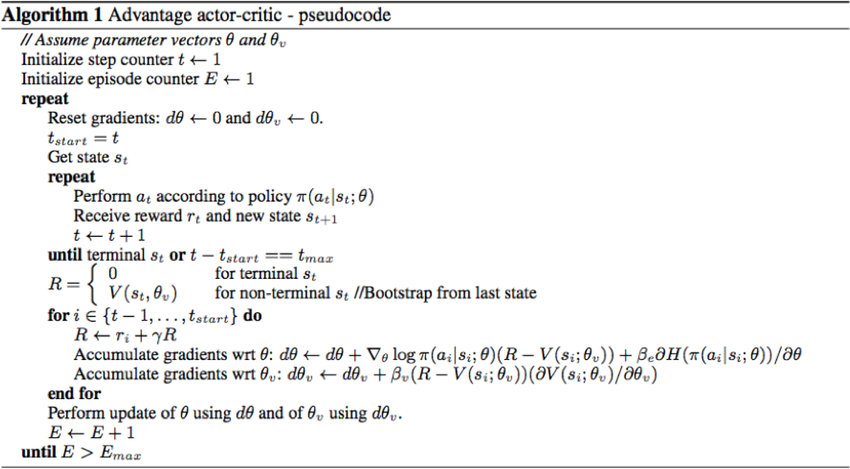
\includegraphics[width=15cm]{assets/a2c-algorithm.jpg}}
    \caption{Algoritam prednosni akter-kritičar (A2C) \cite{A2C}}
    \label{fig:a2c-algorithm}
\end{figure}
